\documentclass[]{scrartcl}
\usepackage[utf8]{inputenc}
\usepackage{graphicx}
\usepackage{amsmath}

\title{Formale Simulation und Verifikation verteilter Algorithmen  \\ Abgabe der Praktikumsaufgabe 1}

\author{Maria Lüdemann und Birger Kamp}

\begin{document}

\maketitle

\begin{abstract}

\end{abstract}

\section{Das Modell als Petrinetz}
Zur Lösung der gestellten Aufgabe haben wir zwei Petri-Netze entwickelt. Beide stellen das Modell da, allerdings wurde das Modell unterschiedlich abstrahiert.

In Variante A wurde der Algorithmus ausführlich implementiert. Dadurch gibt es eine erhöhte Anzahl von Stellen, Transitionen und Kanten.

In Variante B ist der Algorithmus komprimierter und abstrakter dargestellt. Einige der Stellen und Transitionen aus Variante A sind hier zusammengefasst zu finden.
\begin{figure}[htbp]
	\centering
	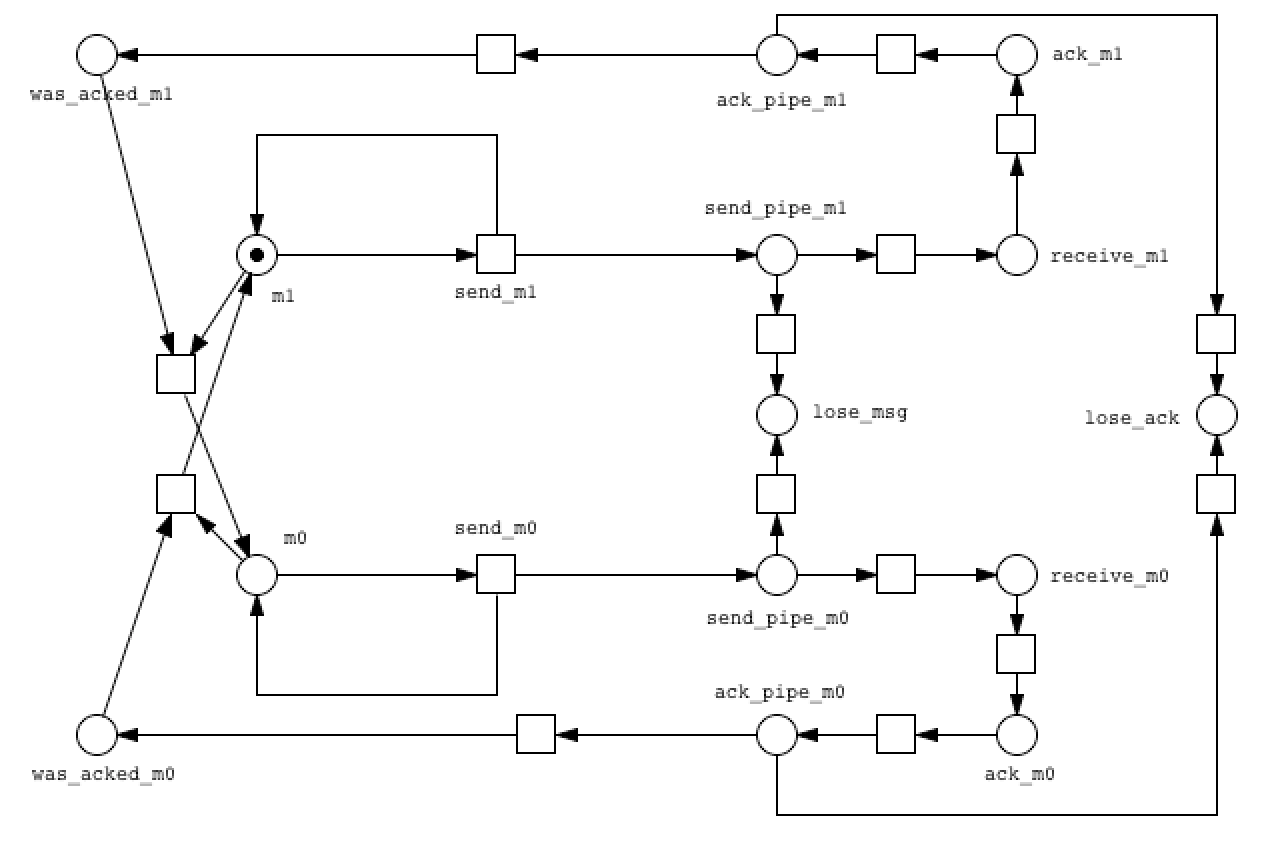
\includegraphics[width=1\linewidth]{petrinet.png}
	\caption{Variante A}
	\label{fig:petri_net_A}
\end{figure}

\begin{figure}[htbp]
	\centering
	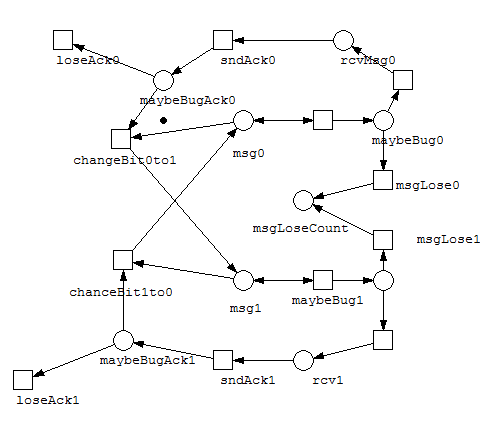
\includegraphics[width=1\linewidth]{altBitPro.png}
	\caption{Variante B}
	\label{fig:petri_net_B}
\end{figure}

\section{Erläuterung der Modellierung}
\subsection{Variante A}
\begin{figure}[htbp]
	\centering
	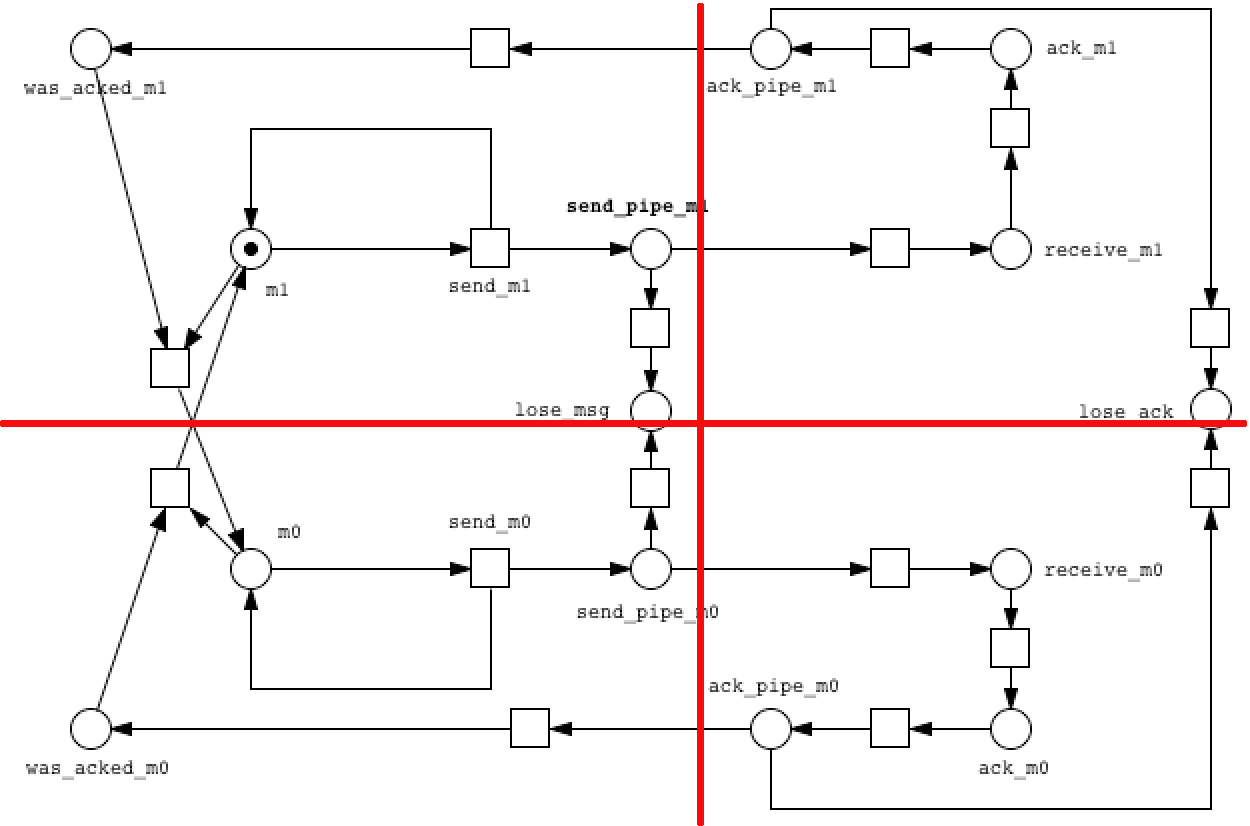
\includegraphics[width=1\linewidth]{petrinet_grid.png}
	\caption{Variante A, in Quadranten eingeteilt}
	\label{fig:petri_net_A_withgrid}
\end{figure}
In Abbildung \ref{fig:petri_net_A_withgrid} wurde das Petri-Netz in Quadranten eingeteilt, um es hier verständlicher beschreiben zu können.

Die Quadranten oben links und unten links sind der Sender des Algorithmus. Der Empfänger ist in den oben rechts und unten rechts abgebildet. Es fällt auf, dass das Netz über die horizontale Achse symmetrisch ist. Das liegt daran, dass die obere Hälfte sich mit dem Senden und Empfangen der Nachrichten mit positivem Kontrollbit kümmert, während der untere Teil für die Nachrichten mit negativem Kontrollbit zuständig sind. Es reicht daher eine der Hälfte in der Funktionsweise zu erklären, da die andere Hälfte sich genauso verhält, nur dass sie dabei eine andere Nachricht behandelt.

In \textit{m1} ist das Start-Token gesetzt, es wird daher zu Beginn eine Nachricht mit positivem Kontrollbit verschickt. Sobald die Nachricht durch die Stelle \textit{send\_m1} verschickt ist, erhält der Initiator \textit{m1} erneut ein Token, dadurch wird ermöglicht, dass die Nachricht erneut verschickt wird, falls der Sender das Empfangen des Empfängers nicht bestätigt bekommt. Außerdem wird die Nachricht "physikalisch" auf die Leitung gelegt, die hier durch die Stelle \textit{send\_pipe\_m1} repräsentiert wird. Dort kann es passieren, dass die Nachricht verloren geht. Sollte die Nachricht nicht verloren gehen, wird sie vom Empfänger in \textit{receive\_m1} erhalten.

Der Empfänger wird nun den Erhalt der Nachricht an den Sender bestätigen. Dazu möchte der Empfänger eine Nachricht senden in der Stelle \textit{ack\_m1}. Die Bestätigungs-Nachricht wird auf die "physikalische" Leitung gelegt, die hier durch die Stelle \textit{ack\_pipe\_m1} dargestellt wird. Dort kann es passieren, dass die Bestätigungsnachricht verloren geht, und der Sender diese nicht erhält. Sollte der Sender die Bestätigung erhalten haben, merkt er sich dies in der Stelle \textit{was\_acked\_m1}.

Sobald der Sender wieder sendebereit ist - wenn also ein Token in \textit{m1} ist - kann der Sender wechseln zum Senden von Nachrichten mit negativem Kontrollbit bzw. der Stelle \textit{m0}. Dort beginnt der Sende-Empfangs-Kreislauf wieder wie bereits für \textit{m1} erklärt.

\subsection{Variante B}
Diese Modellierung beinhaltet zwei autarke Schleifen die das Senden, eventuelle Verlieren und empfangen der Nachrichten modellieren. Diese Schleife gibt es je für die Nachrichten mit dem Kontrollbit 1 und dem für 0. 

\section{Begründung der Korrektheit}
\subsection{Variante A}
Anforderung: \textit{Nachrichten können verloren gehen} \\
Die beiden pipe-Stellen \textit{send\_pipe\_m1} und \textit{send\_pipe\_m0} können ihr Token undeterministsch die Stelle \textit{lose\_msg} oder \textit{receive\_m*}weitergeben. Dadurch ist sichergestellt, dass einige Nachrichten verloren gehen und einige Nachrichten ihr Ziel erreichen. Wieviele Nachrichten wo landen, hängt von der Simulationsumgebung ab.

Anforderung: \textit{Nachrichten enthält Kontrollbit} \\
Das Kontrollbit einer Nachricht wird hier repräsentiert durch die Stellen \textit{m1} und \textit{m0}. Wenn eine dieser Stellen schalten kann, wird die Nachricht mit dem jeweiligen Kontrollbit verschickt.

Anforderung: \textit{Nachricht wird wiederholt bis Empfang bestätigt wurde} \\
Soll eine Nachricht mit Kontrollbit verschickt werden, wird die jeweilige Transition \textit{send\_m*} geschaltet. Diese Transition legt nicht nur die "Nachricht auf die Leitung", sondern teilt dem dazugehörigen \textit{m*} ein Token zu, sodass \textit{m*} wieder das Senden einer Nachricht initiieren kann. Dies wird solange wiederholt bis die Stelle \textit{was\_acked\_m*} schalten kann. Dadurch wird das "Sende-Token" von der aktuellen \textit{m*}-Stelle abgezogen und auf die jeweils andere \textit{m*}-Stelle übertragen, sodass ab dem Zeitpunkt Nachrichten mit dem anderen Kontrollbit verschickt werden.

Anforderung: \textit{Empfänger sendet bei Nachrichterhalt eine Bestätigung an den Sender} \\
Dies wird modelliert durch die Stelle \textit{receive\_m*}. Diese kann schalten, sobald eine Nachricht erhalten wurde. Daraufhin wird in \textit{ack\_pipe\_m*} die Bestätigung "auf die Leitung zum Sender gelegt".

Anforderung: \textit{Empfänger wiederholt Bestätigung bis eine Nachricht mit anderem Kontrollbit ankommt} \\
Der Empfänger bestätigt jede Nachricht, die er bekommt. Sollte der Sender mehrfach Nachrichten mit demselben Kontrollbit schicken, wird für jede der Nachrichten eine Bestätigung an den Sender geschickt.

Anforderung: \textit{Bestätigungen können verloren werden} \\
Sobald eine Bestätigung vom Empfänger "auf die Leitung gelegt" wird - Stelle \textit{ack\_pipe\_m*} - kann die Transition zur Stelle \textit{lose\_ack} geschaltet werden, wodurch die Bestätigungsnachricht "im Netzwerk verloren" wurde.

\end{document}
